\section{Bonus}
General equation of mottion is:
\begin{equation*}
    \begin{split}
        \delta \ddot{x} -3n^2\delta x - 2n\delta \dot{y} = 0\\
        \delta \ddot{y} + 2n\delta \dot{x} = 0\\
        \delta \ddot{z} + 2n\delta \dot{z} = 0\\ 
    \end{split}
\end{equation*}
where:
$$
n = \sqrt{\dfrac{\mu}{r^3}}
$$
above differential equation can be solved in curtis book and final answer is:
\begin{equation*}
    \begin{split}
        \delta x &= 4\delta x_0 + \dfrac{2}{n}\delta \dot y_0 + \dfrac{\delta \dot x_0}{n}\sin(nt)-
        \left(3\delta x_0 + \dfrac{2}{n} \delta \dot y_0\right)\cos(nt)\\
        \delta y &= \delta y_0 -  \dfrac{2}{n}\delta \dot x_0 - 3(2n\delta x_0+ \delta \dot y_0)t + 2\left(3\delta x_0 + \dfrac{2}{n} \delta \dot y_0\right)\sin(nt) + \dfrac{2}{n}\delta \dot x_0\cos(nt)\\
        \delta z &= \dfrac{1}{n}\delta \dot z_0 \sin(nt)+\delta z_0 \cos(nt) \\
    \end{split}
\end{equation*}

$$
\delta \boldsymbol r(t) = \begin{bmatrix}
    \delta x(t)\\
    \delta y(t)\\
    \delta z(t)\\
\end{bmatrix}, \quad \delta \boldsymbol v(t) = \begin{bmatrix}
    \delta u(t)\\
    \delta v(t)\\
    \delta w(t)\\
\end{bmatrix}
$$
$$
\delta \boldsymbol r_0 = \begin{bmatrix}
    \delta x_0\\
    \delta y_0\\
    \delta z_0\\
\end{bmatrix}, \quad \delta \boldsymbol v_0 = \begin{bmatrix}
    \delta u_0\\
    \delta v_0\\
    \delta w_0\\
\end{bmatrix}
$$
$$
\delta \boldsymbol r(t) = \begin{bmatrix}
    \boldsymbol \Phi_{rr}(t)
\end{bmatrix} \delta \boldsymbol r_0 + \begin{bmatrix}
    \boldsymbol \Phi_{rv}(t)
\end{bmatrix} \delta \boldsymbol v_0
$$
$$
\delta \boldsymbol v(t) = \begin{bmatrix}
    \boldsymbol \Phi_{vr}(t)
\end{bmatrix} \delta \boldsymbol r_0 + \begin{bmatrix}
    \boldsymbol \Phi_{vv}(t)
\end{bmatrix} \delta \boldsymbol v_0
$$

$$
\boldsymbol \Phi_{rr}(t) = \begin{bmatrix}
    4 -3\cos(nt) & 0 & 0\\
    6(\sin(nt)-nt) & 1 & 0\\
    0 & 0 & \cos(nt)\\
\end{bmatrix}
$$

$$
\boldsymbol \Phi_{rv}(t) = \begin{bmatrix}
    \dfrac{1}{n}\sin(nt) & \dfrac{2}{n}(1-\cos(nt)) & 0\\
    \dfrac{2}{n}(\cos(nt)-1) & \dfrac{1}{n}(4\sin(nt)-3nt) & 0\\
    0 & 0 & \dfrac{1}{n}\sin(nt)\\
\end{bmatrix}
$$

$$
\boldsymbol \Phi_{vr}(t) = \begin{bmatrix}
    3n\sin(nt) & 2n\sin(nt) & 0\\
    6n(\cos(nt) -1) & 0 & 0\\
    0 & 0 & -n\sin(nt)\\
\end{bmatrix}
$$

$$
\boldsymbol \Phi_{vv}(t) = \begin{bmatrix}
    \cos(nt) & 2\sin(nt) & 0\\
    -2n\sin(nt) & 4n\cos(nt)-3 & 0\\
    0 & 0 & \cos(nt)\\
\end{bmatrix}
$$

The Clohessy-Wiltshire matrices, for $t_f = 8_h$ and $n = 0.0011_{rad/\sec}$.

$$
\boldsymbol \Phi_{rr} = 
\begin{bmatrix}
    1.0361     &    0   &      0\\
    -188.4918 &   1.0000     &    0\\
            0     &    0    &0.9880
\end{bmatrix}
$$


$$
\boldsymbol \Phi_{rv} = 
\begin{bmatrix}
    142  &  22      &   0 \\
    -22 &  -86970 &     0\\
          0    &     0 &   -142
\end{bmatrix}
$$

$$
\boldsymbol \Phi_{vr} = 
\begin{bmatrix}
    -0.0005  & -0.0003   &      0\\
    -0.0001   &      0  &       0\\
          0    &     0 & 0.0070\\
\end{bmatrix}
$$

$$
\boldsymbol \Phi_{vv} = 
\begin{bmatrix}
    0.9880  & -0.3092   &      0\\
    0.0003  & -2.9957  &       0\\
         0   &      0 &   0.9880
\end{bmatrix}
$$

At time $t_f$, Hubble arrives at spaceX, at the origin of the CW frame, which means $\delta \boldsymbol r_f = \delta r_f = \boldsymbol 0$. At $t_f$ we find:
$$
\boldsymbol 0 = \boldsymbol \Phi_{rr}(t_f) \delta \boldsymbol r_0 + \boldsymbol \Phi_{rv}(t_f) \delta \boldsymbol v_0^+
\rightarrow \delta \boldsymbol v_0^+ = -\boldsymbol \Phi_{rr}(t_f)^{-1} \boldsymbol \Phi_{rr}(t_f) \delta \boldsymbol r_0
$$

$$
\delta \boldsymbol v_0^+ = \begin{bmatrix}
    0.9923\\
    -0.3086\\
    0.1232\\
\end{bmatrix}_{m/\sec}
$$

$$
\delta \boldsymbol v_f^- = \boldsymbol \Phi_{vr}(t_f) \delta \boldsymbol r_0 + \boldsymbol \Phi_{vv}(t_f) \delta \boldsymbol v_0^+ = \boldsymbol \Phi_{vr}(t_f) \delta \boldsymbol r_0 + \boldsymbol \Phi_{vv}(t_f) \left(-\boldsymbol \Phi_{rr}(t_f)^{-1} \boldsymbol \Phi_{rr}(t_f) \delta \boldsymbol r_0 \right)
$$


$$
\delta \boldsymbol v_f^- = \begin{bmatrix}
    0.9577\\
    0.9136\\
    0.2465\\
\end{bmatrix}_{m/\sec}
$$

So the change of velocity of Hubble is $|\delta \boldsymbol v_0^- - \delta \boldsymbol v_0^+|$ and the change of velocity of SpaceX is $|\delta \boldsymbol v_f^-|$. The velocity change in this maneuver is not too big. The system is unstable with LQR controller.

\begin{figure}[H]
    \caption{Three dimensional orbit trajectory}
    \centering
    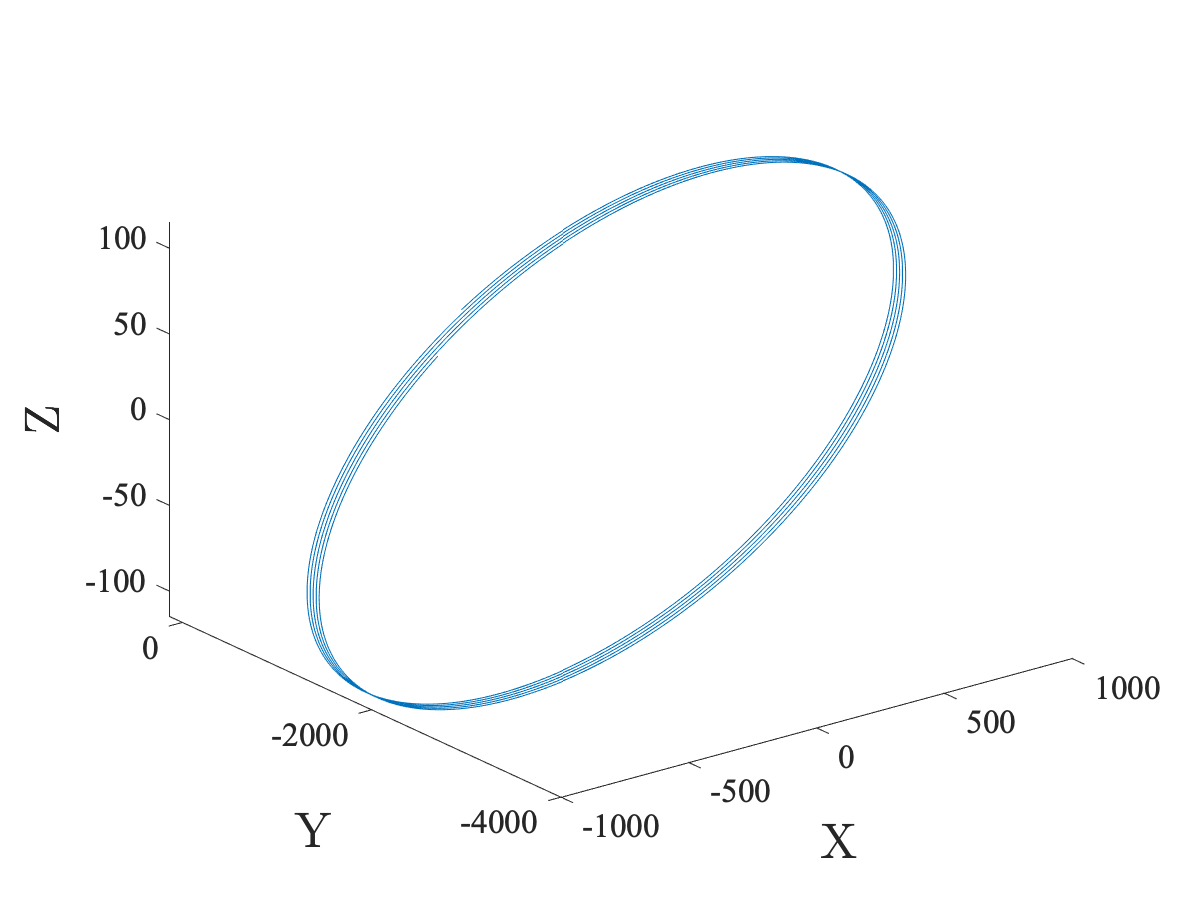
\includegraphics[width=12cm]{../Figure/Bonus/3Dtraj}
\end{figure}

\begin{figure}[H]
    \caption{The orbit trajectory}
    \centering
    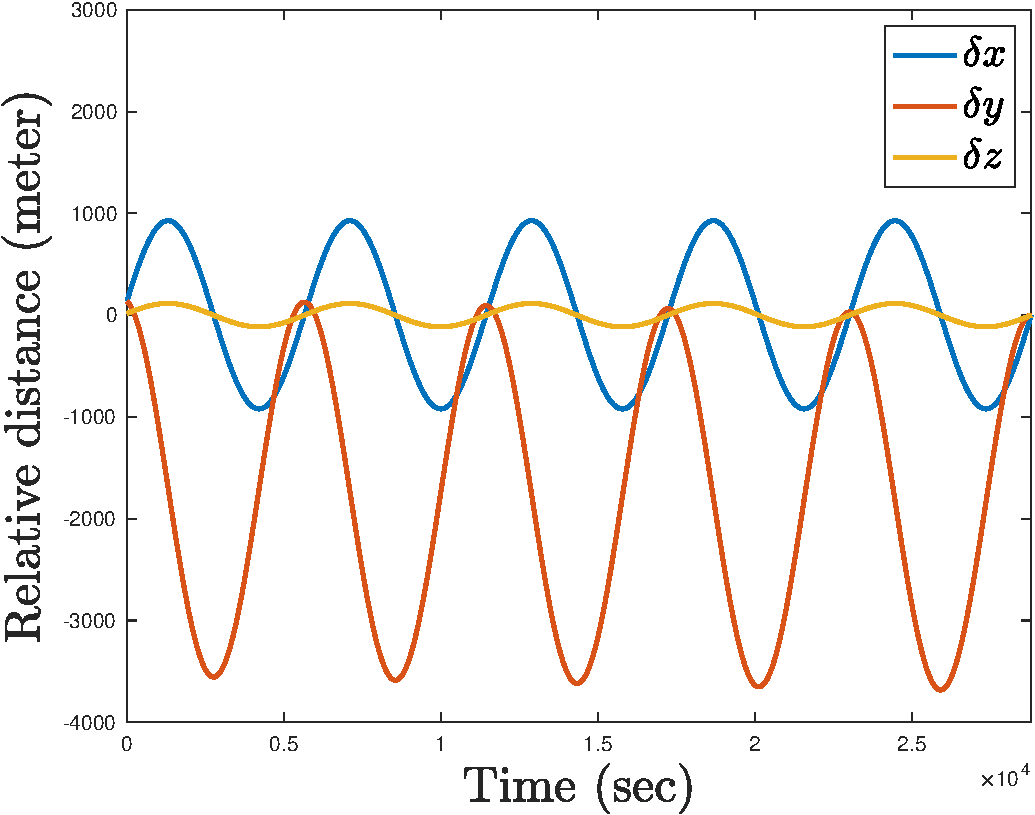
\includegraphics[width=12cm]{../Figure/Bonus/xyz}
\end{figure}